Le but de cette section est d'analyser quels sont les besoins des différents utilisateurs et de trouver quelle est la meilleure manière d'y répondre. Un autre point très important de cette section est le détail des choix technologiques. Je vais donc les passer en revue et les expliquer.
\section{Besoins}

Dans un premier temps, il convient d'identifier quels seront les différents types d'utilisateurs de cette plateforme de quiz. Il y a selon moi deux types bien distincts d'utilisateurs :
\begin{itemize}
    \item Les étudiants
    \item Les professeurs
\end{itemize}

Les premiers utilisent cette plateforme afin de répondre à des quiz. La forme de ces derniers peut varier entre un simple quiz, un drill dans le but de réviser un examen ou finalement l'examen en lui-même. Ils ont donc besoin d'une interface où ils peuvent voir et choisir un quiz parmi tous ceux dont l'accès leurs est autorisé. Il doit pouvoir répondre au quiz et dans le cadre d'un examen ou d'un devoir, il doit pouvoir le rendre. Il doit également pouvoir naviguer dans le quiz.

Les professeurs quant à eux ont des besoins bien différents. Ils veulent principalement créer des quiz avec des questions de plusieurs types tels qu'un QCM, des textes à trous ou encore des questions de code. Ils doivent également pouvoir regrouper leurs étudiants en différentes classes et autoriser cette classe à répondre à certains quiz. De plus, ils peuvent créer et faire passer des examens sur cette plateforme. Dernièrement, ils ont besoin de pouvoir corriger automatiquement certaines questions comme les QCM.

Les besoins ont déjà bien été identifié et décrit par M. Stéphane Bouyiatiotis dans son rapport de TB et je vous invite donc à le consulter. Je vais, pour ma part, me concentrer sur les besoins centrés sur la partie "questionnaire de \emph{drill}".

\subsection{Drill}

Voici nos différents cas d'utilisations concernant la partie \emph{drill} de la plateforme.

\fig[H, width=14cm]{Cas d'utilisation du mode drill}{useCaseDrill.drawio}

Sur ce schéma, on constate que l'utilisation diffère drastiquement entre les deux types d'utilisateurs. Le professeur définit quelles questions pourront être dans le mode \emph{drill}. L'étudiant, quant à lui, veut choisir un sujet de question et y répondre le mieux possible. Il souhaite également que les questions auxquelles il répond de manière incorrecte ou très lente reviennent plus fréquemment que les autres.

\subsection*{Besoins liés au mode drill}
Dans ce tableau, je liste et numérote les besoins des utilisateurs.
\begin{table}[h]
    \begin{center}
        \caption{Besoins des utilisateurs \label{Besoins}}
        \begin{tabular}{|l|l|}
            \hline
            \textbf{} & \textbf{Besoins}                                                            \\
            \hline
            B1        & Choisir le sujet et le nombre de questions                                  \\
            \hline
            B2        & Choisir le temps que va durer le \emph{drill}                               \\
            \hline
            B3        & Lorsqu'on trouve une question facile, elle doit revenir moins fréquemment   \\
            \hline
            B4        & Lorsqu'on trouve une question difficile, elle doit revenir plus fréquemment \\
            \hline
            B5        & Contrôler les questions apparaissant de ce mode                             \\
            \hline
        \end{tabular}
    \end{center}
\end{table}

Une fois ces besoins identifiés, il faut les lier aux différentes fonctionnalités de notre application.

\begin{table}[h]
    \begin{center}
        \caption{Besoins des utilisateurs \label{Besoins}}
        \begin{tabular}{|l|l|l|}
            \hline
            \textbf{} & \textbf{Fonctionnalités}                                                      & \textbf{Besoins lié} \\
            \hline
            F1        & Fournir une interface permettant de personnaliser le \emph{drill}             & B1, B2               \\
            \hline
            F2        & Sélecteur pour choisir le sujet et le nombre de questions                     & B1                   \\
            \hline
            F3        & Sélecteur pour choisir le temps que va durer le \emph{drill}                  & B2                   \\
            \hline
            F4        & Récupérer un nombre défini de questions en fonction de l'utilisateur          & B5                   \\
            \hline
            F5        & Calculer la fréquence de la question en fonction du temps de réponse          & B3, B4               \\
            \hline
            F6        & Calculer la fréquence de la question en fonction de son résultat              & B3, B4               \\
            \hline
            F7        & Editer une question pour la faire apparaitre ou non dans le mode \emph{drill} & B5                   \\
            \hline
        \end{tabular}
    \end{center}
\end{table}



\section{Technologies}
Dans cette sous-section, je vais détailler les différentes technologies qui seront utilisées dans ce projet.
\subsection{Technologies présentes dans l'application}
Je vais brièvement rappeler les choix technologiques qui ont déjà été pris pour ce projet :
\begin{itemize}
    \item Pour le SGBD : MySQL.
    \item Pour le \emph{backend} : le \emph{framework} PHP, Laravel version 8.
    \item Pour le \emph{frontend} : le \emph{framework} javascript, Vue.js version 2.
    \item Pour le style de l'application : Bootstrap et CSS
    \item Pour la connexion à l'application (SSO) : Shibboleth
    \item Système de gestion de version : Github
\end{itemize}

\subsection{Choix technologiques}
Je vais maintenant expliquer et détailler chaque technologie qui sera utilisée au cours de ce projet.

\subsection{MySQL}
MySQL est un système de gestion de bases de données relationnelles (SGBDR) open source et très répandu. Il est bien souvent utilisé dans le développement d'applications ou de sites web pour stocker et récupérer efficacement des données. MySQL utilise le langage de requête SQL pour travailler avec les données. Ce langage permet des fonctionnalités telles que la création de tables, l'insertion, la suppression et la mise à jour des données. Il permet également des fonctionnalités plus avancées comme les jointures qui permettent de récupérer et de combiner les données provenant de plusieurs tables différentes. Ce SGBD a été développé dans le but d'avoir des performances élevées. Sa fiabilité ainsi que sa simplicité à l'utilisation en ont fait l'un des \emph{leaders} dans le monde des SGBD.

Comme le montre le site web de \emph{ranking} de SGBD DB-engines \cite{DBengines}, MySQL est le deuxième SGBD le plus populaire au monde. On constate également qu'il est à cette position depuis plus d'un an. Cela montre sa stabilité.
\begin{center} %TODO : Changer la taille de cette image
    \begin{figure}[H]
        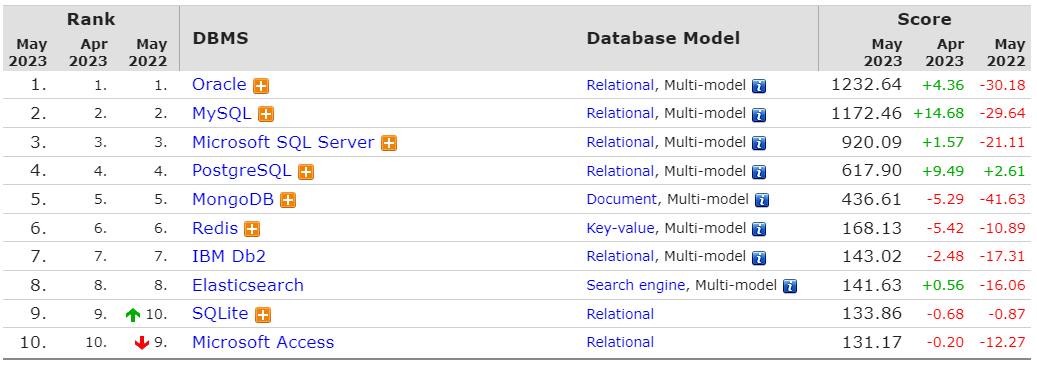
\includegraphics[width=14cm]{./assets/figures/MySQLPopularity.png}
        \caption{Popularité des différents SGBD dans le monde \label{MySQLPopularity.png}}
    \end{figure}
\end{center}
On voit également sur ce classement que les SGBD les deux permiers ont des scores assez similaires et ont tous deux de la marge sur leur concurrent qui occupe la troisième place. Je vais donc brièvement comparer Oracle avec MySQL.

\begin{center}
    \begin{figure}[H]%TODO : Changer la taille de cette image
        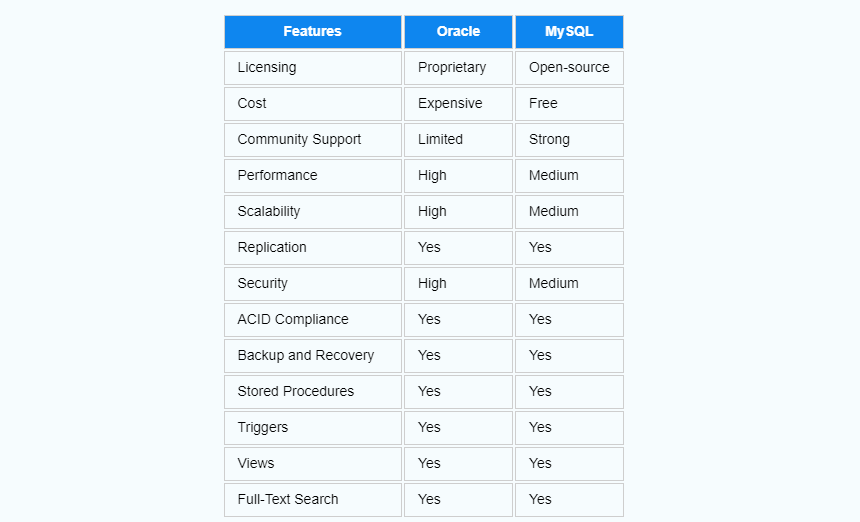
\includegraphics[width=\textwidth]{./assets/figures/OracleVsMySql.png}
        \caption{Comparaison entre Oracle et MySql \label{OracleVsMySql.png}}
    \end{figure}
\end{center}
Cependant comme montré dans l'article du site Integrate.io \cite{Integrate.io} les avantages sont minimes (des performances un peu meilleures et une sécuritée accrue). La licence Oracle étant cependant très onéreuse, ce dernier n'est pas un bon candidat dans le cadre de ce travail de Bachelor.

C'est pourquoi j'ai décidé de rester sur la version 8.0 de MySQL. Cependant, grâce au \emph{framework} Laravel il est extrêmement simple de changer de SGBD. En effet, il suffit de modifier le fichier de configuration. Si dans le futur, nous souhaitons pour une quelconque raison changer de SGBD, ce sera toujours possible et très facile.

\subsection{Laravel}
Laravel est un \emph{framework} \emph{open-source}, écrit en PHP, offrant une structure solide et élégante pour la création d'application et de site web. Le but principal de ce \emph{framework} est de simplifier la création et le développement d'application grâce à des fonctionnalités intégrées. Parmi ces fonctionnalités, on retrouve la gestion de routes, les sessions, l'authentification des utilisateurs ainsi que la gestion de la base de données.
Laravel fournit un ORM (\emph{Object Relational Mapping}), appelé Eloquent permettant de gérer toutes les interactions avec la base de données. Il permet également de choisir avec quel type de SGBD, nous souhaitons travailler et de changer ce dernier très rapidement grâce à des fichiers de configuration.
Il propose également un pattern architechtural très utilisé, le Modèle-Vue-Controller (MVC), que je vais rapidement expliquer.
\begin{center}
    \begin{figure}[H]%TODO : Changer la taille de cette image
        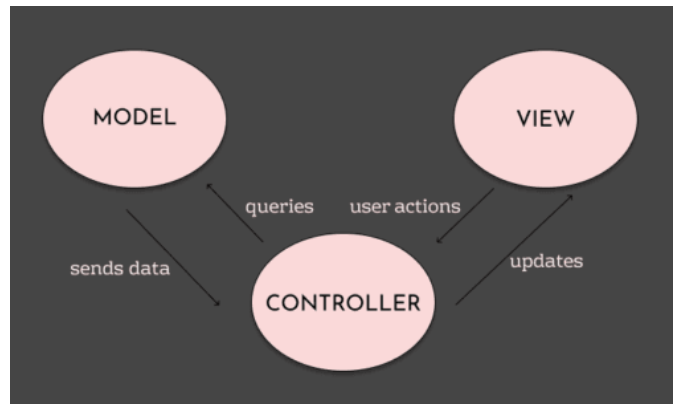
\includegraphics[width=\textwidth]{./assets/figures/MVCExplanation.png}
        \caption{Représentation du MVC \label{MVCExplanation.png}}
    \end{figure}
\end{center}

Sur cette capture, tirée du site Pusher \cite{MVC}, on peut voir les trois parties de ce système et comment elles interagissent.
\begin{itemize}
    \item Le Modèle est la partie responsable de la gestion des données ainsi que de la logique métier. C'est la seule partie du pattern qui interagit avec la base de données. Elle représente les structures de données, et fournit au \emph{Controller} des méthodes pour manipuler les données.
    \item La vue est la partie qui gère de l'interface utilisateur. Elle affiche les données et permet également de récupérer les informations saisies par l'utilisateur notamment au travers de formulaires.
    \item Le \emph{Controller} est la partie qui lie le Modèle et la Vue. Il réagit aux \emph{inputs} de l'utilisateur qui sont transmis par la Vue et va interroger, si nécessaire, le Modèle afin d'y mettre à jours ou récupérer des données. C'est également lui qui détermine quelle est la Vue à afficher à l'utilisateur. C'est le responsable de la logique de l'application.
\end{itemize}
Le MVC permet donc d'avoir une séparation distincte entre les différentes parties de notre application.

Un autre point fort de Laravel est sa gestion des \emph{middleware}. Un \emph{Middleware} est une sorte de filtre qui intervient lorsque les requêtes HTTP arrivent dans notre application. Cela permet notamment d'imposer qu'un utilisateur soit authentifié avant d'accéder à certaines ressources. Ils offrent donc un contrôle accru et centralisent la logique de certaines fonctionnalités.

Laravel est donc l'un des \emph{framework} les plus populaires, simple à prendre en main avec une documentation complète et mise à jour. Il est donc le candidat idéal pour ce projet. De plus, un changement de \emph{framework} imposerait une charge de travail supplémentaire bien trop conséquente.
Je vais donc utiliser la version 10 de Laravel.

\subsection{Vue.js}
Vue.js est un \emph{framework} JavaScript \emph{open-source}, populaire et polyvalent permettant de créer des interfaces utilisateur. Il est principalement utilisé pour le \emph{frontend} d'applications et peut facilement être ajouté à de gros projets. Il propose une approche basée sur les composants qui permettent de créer des portions de codes réutilisable. Grâce à une liaison bidirectionnelle entre les données et l'interface, Vue.js permet de synchroniser, en temps réel, les données entrées par l'utilisateur et leur affichage.

Ce qui permet à Vue.js d'être aussi performant est l'utilisation d'un \emph{DOM} virtuel. Le \emph{DOM (Document Object Model)} est une représentation hiérarchique d'un document HTML sous la forme d'un arbre. Il permet donc à des langages de programmation de modifier le style ou la forme de ce document. Cependant, à chaque changement, le navigateur va mettre à jour l'interface. Cela peut grandement impacter les performances si les modifications sont très fréquentes. C'est pourquoi Vue.js utilise un \emph{DOM} virtuel ou \emph{Virtual DOM}. Il s'agit d'une copie virtuelle stockée en mémoire du \emph{DOM} réel. Lors d'une mise à jour, les changements sont stockés dans le \emph{Virtual DOM}. Vue.js va ensuite comparer le \emph{Virtual DOM} avec le \emph{DOM} réel et n'appliquer que les changements nécessaires. Cela explique pourquoi ce \emph{framework} a des performances relativement élevées.

Pinia est le gestionnaire d'état conseillé pour la version 3 de Vue.js. Il permet de gérer l'état de l'application et de le partager entre les différents composants. Cet outil va nous être très utile au cours de ce projet.

Une autre fonctionnalité très importante de ce \emph{framework} est la capacité de créer des \emph{Singe Page Application} ou une application à page unique. Le concept derrière les SPA est que toute l'application est rendue sur une seule page. La SPA va initialement charger une page puis va dynamiquement changer son contenu en fonction des besoins et volontés de l'utilisateur. Cela permet une expérience utilisateur plus rapide et fluide qu'avec une application classique.

Les principaux concurrents du \emph{framework} Vue.js sont React et Angular. Selon un sondage réalisé par StackOverflow \cite{StackoverflowSurvey} en 2022, React est plus populaire que Vue.js et Angular.
\begin{center}
    \begin{figure}[H]%TODO : Changer la taille de cette image
        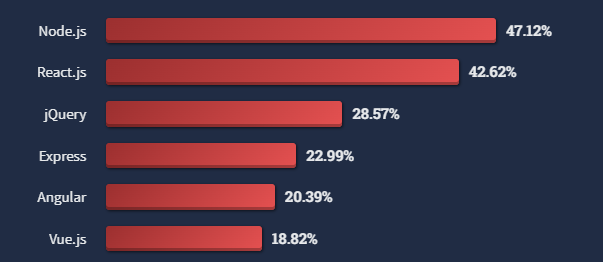
\includegraphics[width=\textwidth]{./assets/figures/VueVSReactVSAngular.png}
        \caption{Popularité des framework web \label{VueVSReactVSAngular.png}}
    \end{figure}
\end{center}

Comme Vue.js, React est un \emph{framework} javascript performant et dispose d'une communauté active. Il aurait été un bon choix de technologie pour ce projet, car plus utilisé dans l'industrie et disposant de plus d'utilisateurs.

Cependant, comme pour Laravel, un changement de \emph{framework} aurait imposé une charge de travail supplémentaire trop importante. De plus, Vue.js est plus simple à prendre en main et à utiliser que React. Il est donc mieux adapté à un projet de cette envergure. Je vais donc utiliser la version 3.0 de Vue.js.

\subsection{TailwindCSS}
TailwindCSS \cite{TailwindCSS} est un \emph{framework} CSS \emph{open-source} très simple à installer et utiliser. Il favorise la création rapide d'interfaces utilisateur personnalisées. Contrairement à son principal concurrent Bootstrap, TailwindCSS ne propose pas de composants prédéfinis. On y retrouve plutôt des classes utilitaires qui permettent de modifier rapidement le style d'un élément. Chaque classe est indépendante et ne représente qu'une fonctionnalité. Par exemple la classe "mb-4" permet d'ajouter une marge sur le bas d'un élément. Cela rend la personnalisation de l'interface utilisateur plus simple et plus rapide. On peut également créer ses propres classes utilitaires.

Un détail important de ce \emph{framework} est qu'il enlève tous les styles de base des navigateurs. Cela permet d'avoir une interface utilisateur cohérente sur tous les navigateurs.

Un autre point fort de ce TailwindCSS est sa communauté active. En effet, TailwindCSS dispose d'une documentation complète et de nombreux exemples.

Les raisons qui ont fait que j'ai choisi TailwindCSS sont sa simplicité d'utilisation, sa capacité de personnalisation. Bootstrap aurait été également un choix tout à fait valable. Cependant, pour avoir déjà travaillé avec ces deux \emph{framework}, j'ai une légère préférence pour TailwindCSS.

\subsection{Keycloak}
Keycloak \cite{Keycloak} est une solution \emph{open-source} de gestion d'identité et d'accès. Cela évite à notre application d'avoir à gérer les différents formulaires d'authentification, d'inscriptions ou de changement de mot de passe. Keycloak propose également une gestion des rôles et des permissions. Cela permet de définir des rôles pour les utilisateurs.

Dans le cadre de ce projet, tous les utilisateurs sont des membres de la HEIG-VD. Les deux choix que nous avions étaient d'utiliser Keycloak (le système de l'école) ou SWITCH edu-ID basé sur Shibboleth (actuellement utilisé dans le projet).

Le grand avantage de Keycloak est la maîtrise complète de l'outil par le service informatique de l'école. Cela permet une meilleure communication et entraide. De plus, Keycloak a déjà été utilisé sur plusieurs projets de l'école, donc sa mise en place sera simplifiée.
C'est pour ces raisons-là que j'ai décidé d'utiliser Keycloak.

\subsection{Github}
Github est une plateforme web de développement collaboratif basée sur Git. Elle facilite énormément la gestion de version de notre code source. De plus, elle favorise grandement la collaboration entre les différents développeurs. Github propose notamment des fonctionnalités de gestion de projet, permettant notamment des créer des tâches et de les assigner à des personnes. Ce qui aide à avoir une meilleure vue d'ensemble du projet.

Github permet également grâce à ses \emph{Github Actions} de créer des \emph{workflows CI/CD} qui permettent d'automatiser certaines tâches. Par exemple, on peut créer un \emph{workflow} qui va automatiquement lancer les tests unitaires à chaque modification du code qui sera poussé sur la plateforme. On peut également créer des \emph{Github Actions} qui vont déployer automatiquement notre application sur un serveur.

Github est la plateforme de gestion de version la plus populaire et la plus utilisée dans le monde. Selon les statistiques de l'article de Radix \cite{Radix}, Github aurait environ 56 millions d'utilisateurs contre 31 millions pour Gitlab. Avec son système de \emph{stars} et son côté social, Github est la plateforme idéale pour un projet open-source.

Toutes ces raisons font que Github est la plateforme de gestion de version choisie pour ce projet.
\newpage
\subsection{Récapitulatif des technologies}
Dans le tableau ci-dessous, vous pouvez trouver la liste de toutes les technologies qui sont utilisées dans le cadre de ce projet ainsi que leur version.
% Fais un tableau avec toutes les technologies utilisées dans le projet
\begin{table}[h]
    \begin{center}
        \caption{Technologies utilisées lors du projet \label{stack}}
        \begin{tabular}{|l|l|}
            \hline
            \textbf{Technologie} & \textbf{Version} \\
            \hline
            MySQL                & 8.0              \\
            \hline
            PHP                  & 8.2.6            \\
            \hline
            Composer             & 2.5.5            \\
            \hline
            Laravel              & 10               \\
            \hline
            Node                 & 18.15.0          \\
            \hline
            NPM                  & 9.5.0            \\
            \hline
            Vue.js               & 3                \\
            \hline
            Tailwind CSS         & 3.3.1            \\
            \hline
            WSL                  & 2                \\
            \hline
            Docker               & 20.10.22         \\
            \hline
            Ubuntu               & 22.04.2 LTS      \\
            \hline
            Keycloak local       & 21.1             \\
            \hline
            Github               & -                \\
            \hline
        \end{tabular}
    \end{center}
\end{table}